\subsubsection{05.12.14}

\begin{enumerate}
	\item The time of beginning and ending of the meeting:
	16:00 - 20:00
	\item Purposes of the meeting:
	\begin{enumerate}
	  \item To install П-shaped rib of rigidity.
	  
	  \item To measure the inner space of robot and choose optimal sizes of bucket.
	  
    \end{enumerate}
	\item Work, that has been done:
	\begin{enumerate}
	  \item П-shaped rib of rigidity was installed.
	  
	  \begin{figure}[H]
	  	\begin{minipage}[h]{0.2\linewidth}
	  		\center  
	  	\end{minipage}
	  	\begin{minipage}[h]{0.6\linewidth}
	  		\center{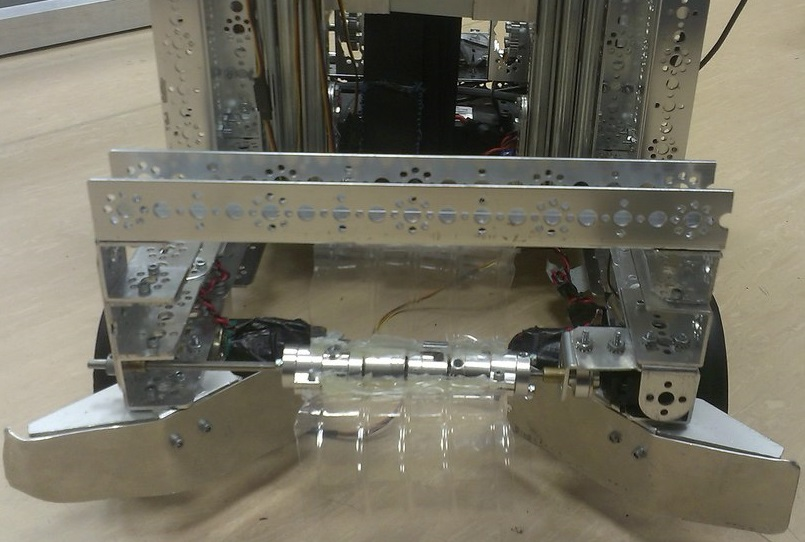
\includegraphics[scale=0.3]{days/05.12.14/images/01}}
	  		\caption{П-shaped rib of rigidity}
	  	\end{minipage}
	  \end{figure}
	  
	  \item We measured the space allocated for bucket. Optimal sizes of bucket were choose.
	  
	  \item Programme of autonomous period was improved. Function that convert reading of encoder to centimeters was removed. It allowed solve the problem with turning to parking zone.	  
	  
    \end{enumerate}
    
	\item Results:  
	\begin{enumerate}
	  \item П-shaped rib of rigidity was installed.
	  
	  \item Programme of autonomous period was improved.
	  
    \end{enumerate}
    
	\item Tasks for the next meetings:
	\begin{enumerate}
	  \item To create the drawing for new bucket.
	  
	  \item To choose and buy the material for bucket.
	  
    \end{enumerate}     
\end{enumerate}
\fillpage